\documentclass[letterpaper,12pt]{article}
\usepackage[margin=64pt]{geometry}
\usepackage{amsthm}
\usepackage{amsmath}
\usepackage{amssymb}
\usepackage{parskip}
\usepackage{graphicx}
\usepackage{enumerate}
\usepackage{hyperref}
\usepackage{listings}
\newcommand{\transpose}{^{\mbox{\tiny T}}}


\begin{document}
\thispagestyle{empty}

\hrule \vspace{0.5em}
\noindent {\bf CFRM 462: Introduction to Computational Finance and Econometrics} \hfill Homework 2 \newline \hrule

\vspace{1em}

\begin{enumerate}
\item
\subitem{a)} 1 - pnorm(0.1,mean = 0.05, sd = 0.1) = 0.3085375
\subitem{b)} pnorm(-0.1,mean=0.05,sd = 0.1) = 0.0668072
\subitem{c)} pnorm(0.15,mean=0.05,sd = 0.1) - pnorm(-0.05,mean=0.05,sd = 0.1) = 0.6826895
\subitem{d)} qnorm(.01,mean=0.05,sd = 0.1) = -0.1826348
\subitem{e)} qnorm(.05,mean=0.05,sd = 0.1) = -0.1144854
\subitem{f)} qnorm(.95,mean=0.05,sd = 0.1) = 0.2144854
\subitem{g)} qnorm(.99,mean=0.05,sd = 0.1) = 0.2826348
\item 
x.vals = seq(-0.25,0.35,length = 150)*0.1 + 0.05

plot(x.vals,dnorm(x.vals,mean = 0.05,sd = 0.1),type = "l",lwd = 2, col = "blue", xlab = "x", ylab = "pdf",main = "Combined PDF",ylim = c(0,8))

lines(x.vals,dnorm(x.vals,mean = 0.025,sd = 0.05))\\
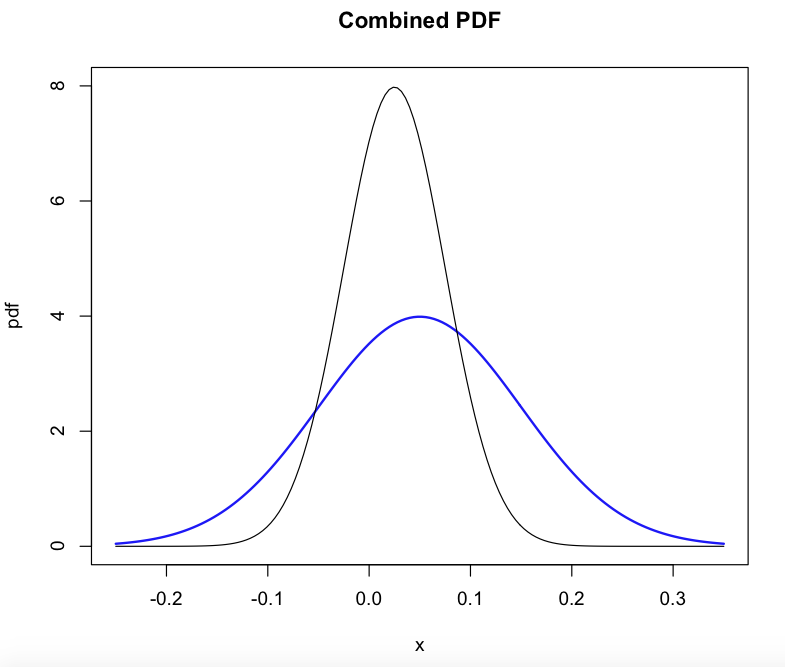
\includegraphics[scale = 0.5]{PDF} \\
Microsoft has more risk than Starbucks, which means a higher potential return. However, Starbucks has a less risk which means your expected return will be lower.

\item 
\begin{lstlisting}[language = R]
> mu.R = 0.04
> sd.R = 0.09
> 
> w0 = 10000
> 
> q.01.R = mu.R + sd.R *qnorm(0.01)
> q.05.R = mu.R + sd.R *qnorm(0.05)
> 
> var.01 = abs(q.01.R * w0)
> var.05 = abs(q.05.R * w0)
> var.01
[1] 1693.713
> var.05
[1] 1080.368
\end{lstlisting}
\item Continuously Compounded Monthly and Annual Var
\begin{lstlisting}[language = R]
e.01.R = exp(mu.R + sd.R * qnorm(0.01)) - 1
e.05.R = exp(mu.R + sd.R * qnorm(0.05)) - 1

e.Var.01 = abs(e.01.R * w0)
e.Var.05 = abs(e.05.R * w0)

> e.Var.01
[1] 1558.046
> e.Var.05
[1] 1024.055
\end{lstlisting}
\subitem{b)}

\begin{lstlisting}
> abs(e.01.R * 12 * w0)
[1] 18696.55
> abs(e.05.R * 12 * w0)
[1] 12288.66
\end{lstlisting}

\item \begin{lstlisting}
x.vals = seq(-5,5, length = 100)
pos = seq(0,5,length = 100)

plot(x.vals,dt(x.vals,1),type = "l", lwd = 2, col = 1, ylim = c(0,0.6), xlab = "X", ylab = "PDF", main = "Student T Distribution")
lines(x.vals,dt(x.vals,2),type = "l", lwd = 1, col = 2)
lines(x.vals,dt(x.vals,5),type = "l", lwd = 1, col = 3)
lines(x.vals,dt(x.vals,10),type = "l", lwd = 1, col = 4)

#Chi Squared
plot(pos,dchisq(pos,1),type = "l", lwd = 1, col = 5, xlab = "X", ylab = "PDF", main = "Chi-Squared")
lines(pos,dchisq(pos,2),type = "l", lwd = 1, col = 6)
lines(pos,dchisq(pos,5),type = "l", lwd = 1, col = 7)
lines(pos,dchisq(pos,10),type = "l", lwd = 1, col = 8)
\end{lstlisting}
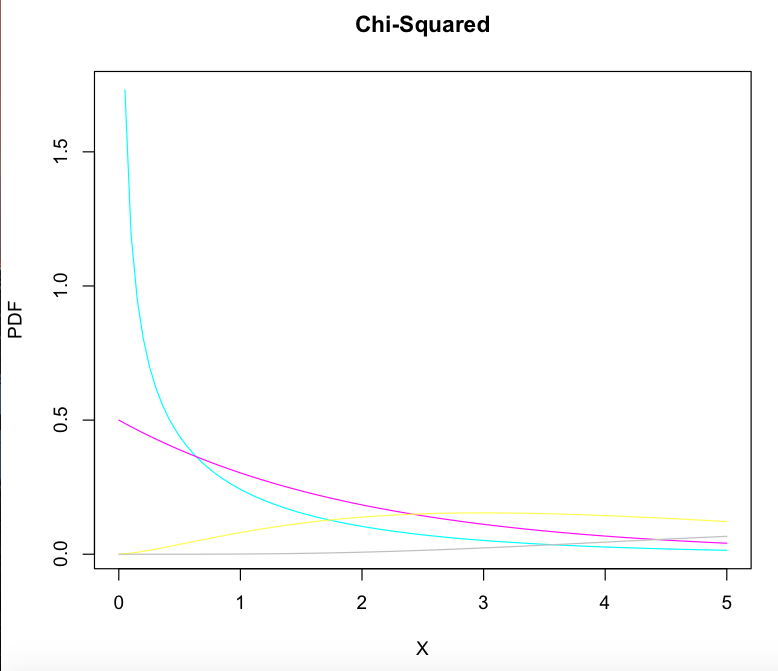
\includegraphics[scale = 0.4]{Chi-Squared} \\
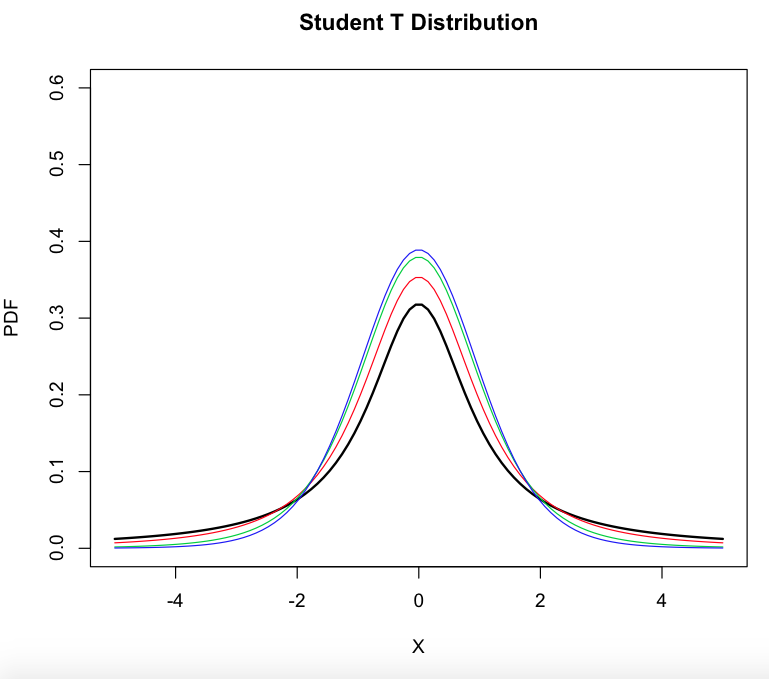
\includegraphics[scale = 0.4]{T-Distribution}

\item \begin{lstlisting}[language = R]
e.x = 1*.3 + 2*.3 + 3 * 0.4
var.x = 1*.3 + 4*.3 + 9 * .4 - E.x^2
sd.x = sqrt(var.x)

e.y = 1 * 0.2 + 2*0.3 + 3*0.5
var.y = 1* 0.2 + 4 * 0.3 + 9 * 0.5 - e.y^2
sd.y = sqrt(var.y)

e.xy = (1*1*0.1) + (1*2*0.2) + (2*1*0.1) + (2*3*0.2) + (3*2*0.1) + (9*0.3)

cov.xy = e.xy - e.y*e.x
cor.xy = cov.xy/(sd.x*sd.y)
> answers <- c(e.x,var.x,sd.x,e.y,var.y,sd.y)

\end{lstlisting}
\subitem{a)} 2.1000000 0.6900000 0.8306624 2.3000000 0.6100000 0.7810250
\subitem{b)} 0.37, 0.5703117
\subitem{c)} No they are not independent. 
\[
P(y = 1 | x = 1) = \frac{P(x = 1, y = 1)}{P(x = 1)} = \frac{.1}{.3}
\neq P(y = 1) = 0.2
\]

\item \begin{lstlisting}
#Problem 7
b.amzn = 38.23
b.costco = 41.11

s.amzn = 41.29
s.costco = 41.74

#Simple Monthly Return
r.amzn = (s.amzn - b.amzn)/b.amzn
r.costco = (s.costco - b.costco)/b.costco

> r.amzn
[1] 0.08004185
> r.costco
[1] 0.01532474

#CC Return
cc.amzn = log(s.amzn/b.amzn)
cc.costco = log(s.costco/b.costco)

> cc.amzn
[1] 0.07699979
> cc.costco
[1] 0.0152085

#dividend
div = 0.1
rd.costco = (s.costco + div)/(b.costco) - 1
rd.yield = div/b.costco

> rd.costco
[1] 0.01775724
> rd.yield
[1] 0.002432498

#annualized
annual.amzn = (1+r.amzn)^12 - 1
annual.costco = (1+r.costco)^12 - 1

> annual.amzn
[1] 1.519341
> annual.costco
[1] 0.2002166

annual.amzn.cc = 12 * cc.amzn
annual.costco.cc = 12 * cc.costco

> annual.amzn.cc
[1] 0.9239975
> annual.costco.cc
[1] 0.182502

x_a = 0.8
x_c = 0.2

r.combined = x_a * r.amzn + x_c * r.costco
cc.combined = log(1+r.combined)

> r.combined
[1] 0.06709843
> cc.combined
[1] 0.06494322

> R_e
[1] -0.1333333
> R_uk
[1] 0.125
> R_us
[1] -0.025
\end{lstlisting}
\[
	R_e = \frac{e_1 - e_0}{e_0}
\]
\[
	R_uk = \frac{uk_1 - uk_0}{uk_0}
\]
\[
	R_{us} = (1 + R_e)(1+R_uk) - 1
\]


\item \[
	cov(R_t,R_{t-1}) = E[R_tR_{t-1}] - E[R_t]E[R_{t-1}]
\]
\[
	0 = E[R_tR_{t-1}] - E[R_t]E[R_{t-1}]
\]
\[
	E[R_tR_{t-1}] = E[R_t]E[R_{t-1}]
\]
\[
	R_t \sim N(\mu,\sigma^2) \therefore E[R_t] = \mu
\]
\[
	\implies E[R_tR_{t-1}] = \mu^2
\]
\[
	E[R_t(2)] = E[(1+R_t)(1+(R_{t-1}) - 1]
\]
\[
	(1 + E[R_t])(1+E[R_{t-1}]) - 1
\]
\[
	\implies (1+\mu)^2 - 1
\]

No $R_t(2)$ is not normally distributed since it is the product of two normal distribution. 

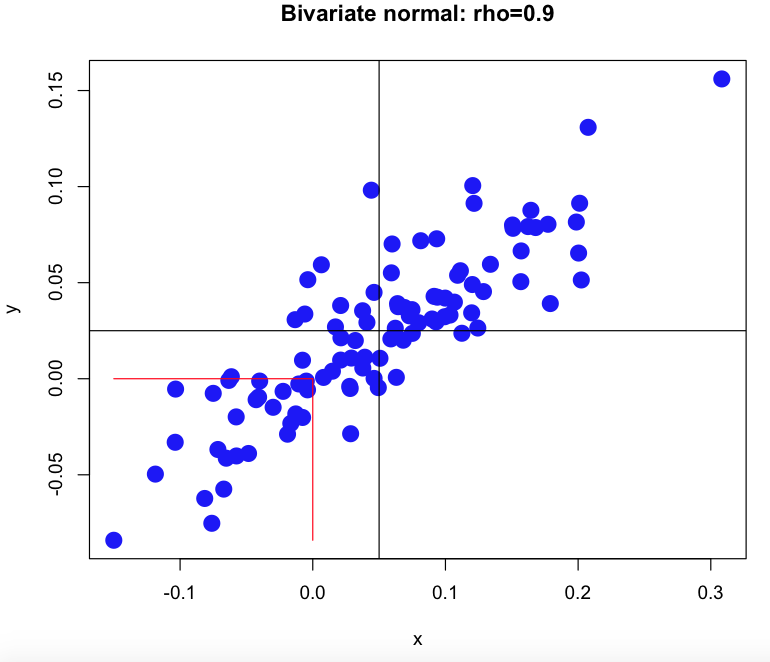
\includegraphics[scale = 0.5]{Positive} \\
The graph has a positive linear relationship and the joint probability is 0.245 \\
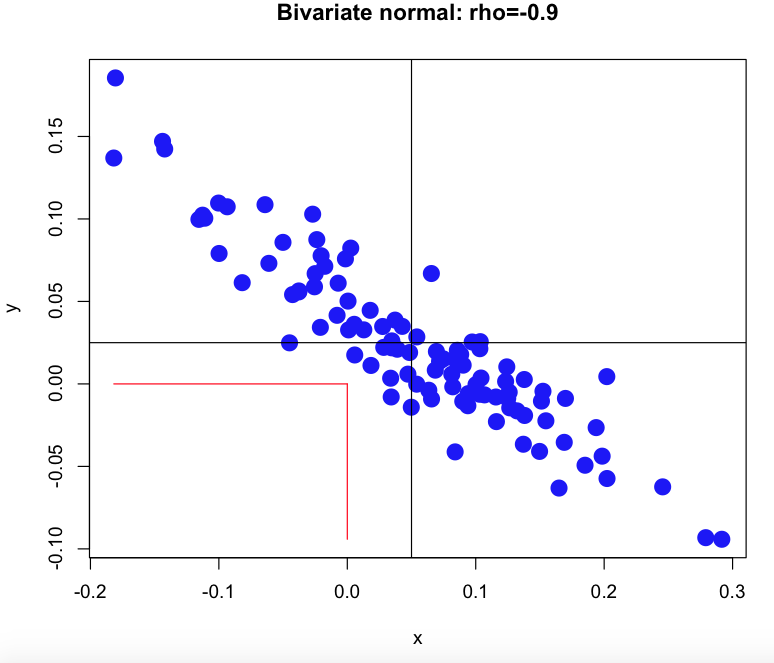
\includegraphics[scale = 0.5]{Negative} \\
The graph has a negative linear relationship and the joint probability is 0.000803 \\ 
\includegraphics[scale = 0.5]{"No Association"} \\
The graph has no correlation and the joint probability is 0.0952
\end{enumerate}

\vfill \hrule \vspace{2mm} \centerline {\tt \tiny http://computational-finance.uw.edu}
\end{document}